% Chapter Template

% Article Title: On the Structural Analysis of Polysaccharide-Networks by Transmission Electron-Microscopy: Comparison with SAXS
\chapter{Validation of Transmission Electron-Microscopy Imaging: Comparison with SAXS}
% chapter title

\label{Chapter-TEMSAXS} % Change X to a consecutive number; for
% referencing this chapter elsewhere, use \ref{ChapterX}

\lhead{Chapter 3. \emph{TEM-SAXS Comparison}}
% Change X to a consecutive number; this is for the header on each page - perhaps a shortened title

\section{Abstract}
\noindent
Polysaccharide gels assembled from the anionic biopolymers pectin and carrageenan have been studied using transmission electron microscopy (TEM). Gels were formed in several different ways: for pectin, hydrogen bonding was used to form junction-zones between strands, while for carrageenan systems several different ion types were used to form ionotropic networks. Using this approach, several distinct network architectures were realized. In addition to preparing gelled samples for electron microscopy, a set of samples was taken without performing the additional treatment necessitated by the TEM measurements, and these were studied directly by small-angle x-ray scattering (SAXS). Taking careful consideration of the relative merits of different image sizes and available processing techniques, the real-space images acquired by TEM were used, via radial integration of the Fourier transform, in order to produce simulated scattering patterns. These intensity-versus-wavevector plots were compared with the results of SAXS experiments carried out on the unadulterated gels using synchrotron radiation. While information regarding chain thicknesses and flexibilities was found to be modified by labeling and by changes in the dielectric constant and mechanical properties of the surroundings in the TEM, the studies carried out here show that careful protocols can produce datasets where information acquired above around 20 nm is broadly consistent with that obtained by SAXS studies carried out on unadulterated samples. The fact that at larger length scale the structure of these water-rich networks seems largely preserved in the TEM samples suggests that 3D TEM tomography experiments carried out with careful sample preparation will be valuable tools for measuring network architecture and connectivity; information that is lost in SAXS owing to the intrinsic averaging nature of the technique.

\section{Introduction}

Visualizing structures smaller than the wavelength of visible light is an important goal of benefit to a plethora of scientific disciplines, as recognized by the recent award of the Nobel Prize in Physics for developments in near-field imaging. Structural studies can be performed in real or reciprocal space. In many cases reciprocal space techniques, (scattering or diffraction), can be performed down to atomic length-scales using electrons, neutrons or x-rays. However, for some systems real-space information is paramount due to the difficulty of retrieving phase information in the reciprocal domain without extra experimental effort. Such phase information can provide valuable insights into the spatial arrangement of constituents. Spatial information is especially important when studying systems such as dispersions and polymer networks. The study of polymeric networks in soft condensed matter research typically employs real-space microscopy techniques due to the fact that the detailed spatial architecture can play a critical role in giving rise to the bulk mechanical \cite{onck_alternative_2005, lindstrom_finite-strain_2013} and transport \cite{walther_influence_2006,loren_dendrimer_2009} properties of the system, while scattering techniques average over heterogeneities in network connectivity. 


Fibrillar proteins such as actin and collagen have been at the center of extensive studies into the underlying structure-function relationships in these complex materials \cite{broedersz_filament-length-controlled_2012}. Typically these systems assemble into networks on length-scales where suitably stained individual strands can be visualized with wide-field fluorescence or confocal microscopy. Images of networks obtained in this way are generally considered to be minimally perturbed and faithful representations of the unstained samples\cite{magatti_modeling_2013}. In contrast, networks assembled from polysaccharides typically form architectures on length-scales reduced by around an order of magnitude compared with fibrillar proteins and, as such, their real-space visualization relies heavily on electron microscopy (EM) techniques. Recent technological advances have produced  EM techniques that are generally considered to faithfully preserve the structures of hydrated proteins without the requirement for contrast agents \cite{dohnalkova_imaging_2011}. However, for polymeric systems such as polysaccharides the limited phase contrast offered by these biomolecules typically requires invasive sample preparation. Even with systematic application the spectre of preparation artifacts is often raised. Despite this, few studies have been carried out in order to assess the level of confidence that can be assigned to different aspects of polysaccharide networks obtained using different EM techniques.

Previous TEM measurements have been performed on a number of different polysaccharide networks such as alginate, carrageenan and pectin\cite{lundin_rheology_1997, brun_texture_2011, domozych_pectin_2014} and in many of the different systems significant qualitative differences between networks can be seen, although few quantitative measurements have been performed.

In this work, several distinct network architectures were realized from two well-known gelling polysaccharides; pectin and carrageenan; key structural polysaccharides in land and marine plants respectively. In addition to preparing gelled samples for electron microscopy, a set of samples was taken without performing the additional treatment necessitated by the imaging measurements. These were studied directly by small-angle x-ray scattering (SAXS), and the results compared.


\section{Materials and methods}
\textbf{Pectin: }The gelation method exploited herein has been described in detail previously \cite{mansel_zooming_2015}. To summarize: a commercially available pectin sample that had a high degree of methylesterification (DM) (78\%) was modified using a processive pectin methyl esterase (PME) extracted from oranges and sourced from Sigma, to obtain a block-wise sample with DM of around 40\%, and the resulting polymer freeze dried. The polymeric fine structure was measured using capillary electrophoresis as described elsewhere. Subsequently a solution was made by dissolving \SI{0.02}{\g} of the freeze-dried pectin in \SI{1.5}{\ml} of deionized water. Next \SI{0.16}{\g} of glucono delta-lactone (GDL) was dissolved in water and mixed with the pectin solution as quickly as possible, in order to minimize any hydrolysis of GDL occurring before mixing, while being careful not to form bubbles. This solution was then loaded into the requisite sample cells for TEM or SAXS.

\textbf{Carageenan: }Ion-exchanged sodium carageenan samples were provided by Dupont. Relevant salt solutions (30 mM KCl  or 300 mM NaCl) were first made by dissolving the required amount of salt in a volumetric flask and using millQ water. The required amount of dry carrageenan in order to produce 1\% w/w solutions was then weighed out and subsequently suspended in the relevant salt solution. The solutions were then heated to \SI{60}{\degreeCelsius} while stirring until all powder was dissolved. This solution was then loaded hot into the requisite sample cells for TEM or SAXS and gels formed on cooling to room temperature.

\textbf{TEM: }Gels were fixed with 0.1\% Ruthenium Red and phosphate buffered 2.5\% glutaraldehyde prior to dehydration in a graded ethanol series and embedding in an epoxy resin (ProCure 812, ProSciTech, Thuringowa, Australia). Fixation mechanisms for aldehydes are known to some extent from protein crystallographic studies, where in particular covalent bonding with lysine residues is employed \cite{wine_elucidation_2007}, but no comparable studies exist for polysaccharides. We found that Ruthenium Red was essential for maintaining sample integrity during dehydration. We observed that this was due to the formation of a skin on the gel pieces. The role of glutaraldehyde in preserving or altering structure is unknown but our observations suggest that there is no effect on the bulk structure down to the level of individual molecules, where some combination of fixation and staining changes the native morphology. Indeed, some deviation from native structure must be expected due to the use of one or more of these reagents. Sections with nominal thickness of 150 nm were cut with an ultramicrotome and post-stained with 2\% uranyl acetate prior to visualisation. Previous work using tomography to acquire images from pecin gels in 3D \cite{mansel_zooming_2015} suggests that this post-staining is effective throughout the section thickness. Imaging areas were pre-irradiated for 15 minutes at low magnification prior to image acquisition. Two-dimensional micrographs were recorded on a JEOL JEM-1400 transmission electron microscope with a $\text{LaB}_6$ cathode operated at 120 kV under low-dose conditions with synchronised beam blanking and acquisition. Projection images were collected on a Gatan Ultrascan 2K$\times$2K CCD with a pixel size of \SI{0.86}{\nm} (nominal magnification of 12 000X).

\textbf{SAXS:} SAXS experiments were performed at the Australian Synchrotron on the SWAXS beamline where samples were prepared in $\sim$\SI{1.5}{\mm} quartz glass capillary tubes (purchased from Hampton Research or capillarytubes.co.uk) and irradiated with \SI{11}{\keV} radiation. For this high-flux undulator-beamline, a slit was used to attenuate the beam and multiple (typically 10) 1 or 2 second exposures were averaged over in order to increase the signal-to-noise ratio. The sample was translated between exposures in order to prevent beam damage. Scattered radiation was collected using a Dextrus Pilatus 1M detector, with sample to detector distances of 7179 mm and 719 mm.

\textbf{Image Analysis:}
Using the FFT of real space images in order to obtain results that are easily comparable to scattering data, (intrinsically measured in the reciprocal space), has been utilized previously with two \cite{tanaka_application_1986} and three dimensional images \cite{takahashi_real_2003} for different systems. For this study we utilize the Fourier transform of large two dimensional images (montages) in a quest to access larger length scales (lower scattering vectors) than would be possible using reconstructed three dimensional tomograms.


In-house software\footnote{https://github.com/phcerdan/FFTRadialIntensity\label{code}} written in C++11, utilizing the image analysis open source library ITK \cite{johnson_itk_2017}, was used to measure the reciprocal-space properties of the images and directly compare these to SAXS data. Following the principles of open science and reproducibility, the code and data used in this article can be found in a public repository\textsuperscript{\ref{code}} under an MPL (free) license. A terminal based executable for batch processing, and a graphical interface for visualization of the analysis process are provided, as well as instructions of how to build the code to run on different operating systems.

\begin{figure}[!ht]
  \centering
  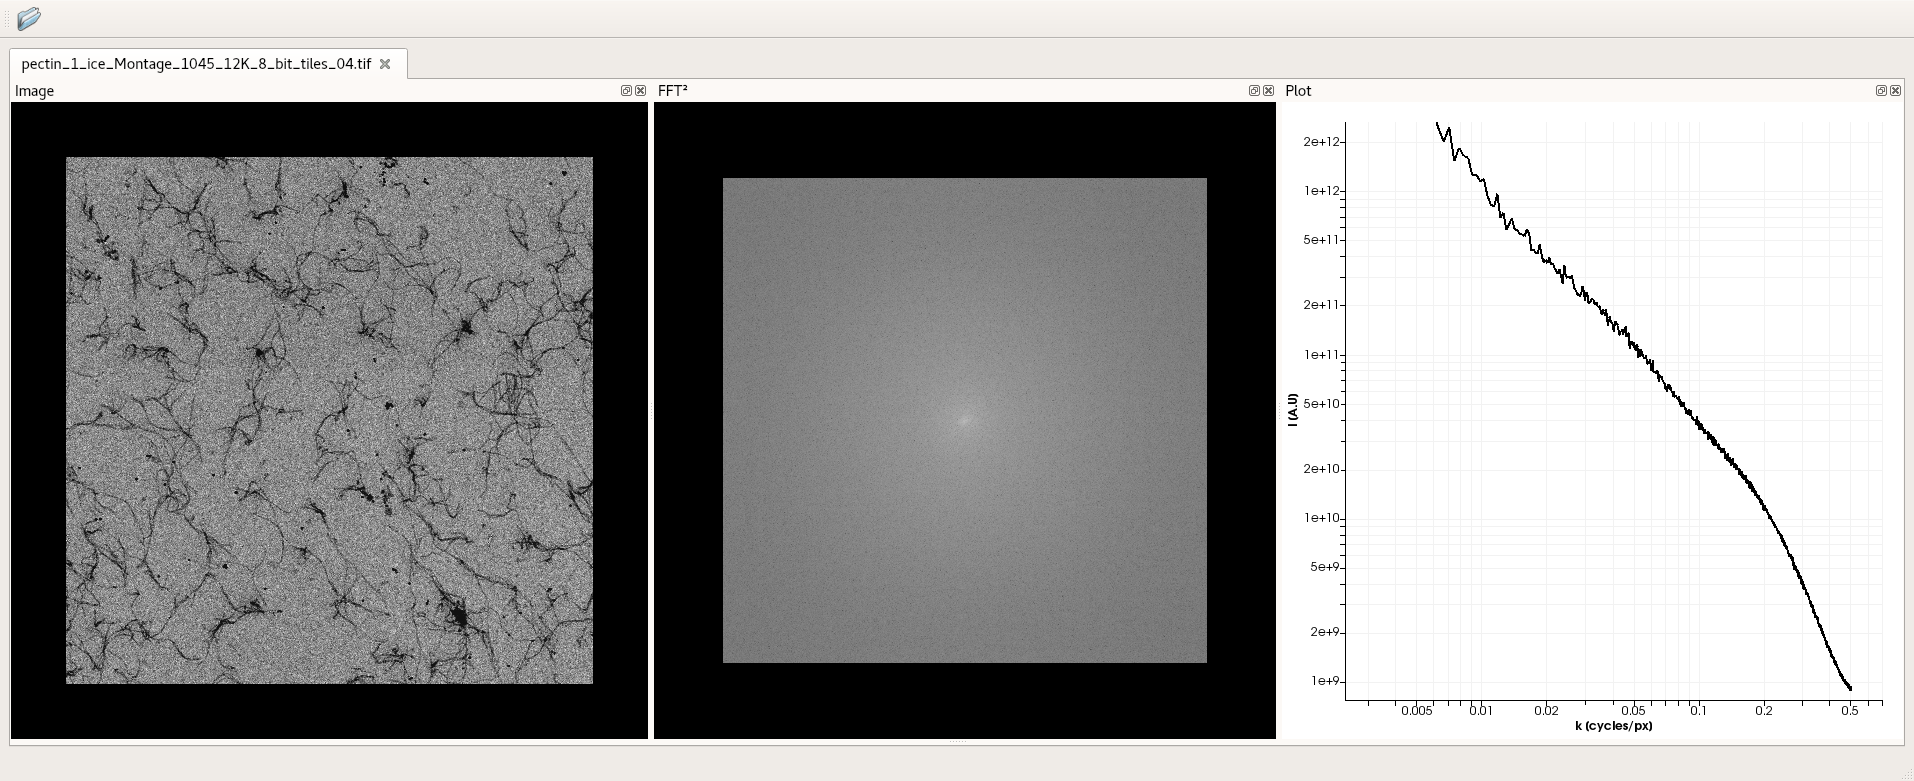
\includegraphics[width=0.99\linewidth]{Figures/chapter-temsaxs/software_screenshot_stretch.png}
  \caption{The Graphical User Interface (GUI) of the image analysis software developed herein. A non-interactive interface is also provided for batch processing, along with python scripts for plotting and manipulation of the generated data.}\label{fig:fig_gui}
\end{figure}


Fundamentally the measured pixel intensity in the images, $I(\bm{r})$, at position $\bm{r}$, is proportional to the difference of refractive index $I(\bm{r}) \propto \delta n(\bm{r})$  to a good approximation, so that the power spectrum $P(\bm{k})$ of the Fourier Transform ($\mathscr{F}\{I(\bm{r})\} = F(\bm{k})$)  (Eq.~\ref{eq:power_fft}) is also proportional to the scattering intensity $S(\bm{k})$ (eq.~\ref{eq:power_scattering_relation}) obtained by light scattering experiments \cite{tanaka_application_1986}.

\begin{equation}\label{eq:power_fft}
  P(\bm{k}) = |F(\bm{k})|^2 = \int_{v}\langle I(\bm{r})I(\bm{0})\rangle \exp(-j\bm{k}.\bm{r})d\bm{r}
\end{equation}
\begin{equation}\label{eq:power_scattering_relation}
   P(\bm{k}) \propto S(\bm{k}) \propto \int_{v}\langle n(\bm{r})n(\bm{0})\rangle \exp(-j \bm{k}.\bm{r})d\bm{r}
\end{equation}
Eq.~\ref{eq:power_fft} uses the Convolution theorem $\mathscr{F}\{I\} \cdot \mathscr{F}\{I\} = \mathscr{F}\{I*I\} $, with $\langle I(\bm{r})I(\bm{0})\rangle = \int I(\bm{s} - \bm{r})I(\bm{s}) d\bm{s}$.

\noindent Here $\bm{k}$ is the angular reciprocal space vector:
\begin{equation}\label{angular_freq}
  \bm{k} = 2\pi \cdot \bm{\xi}
\end{equation}
Most digital Fourier Transform implementations work with non-angular $\bm{\xi}$ variables, so it is necessary to apply a factor of $2\pi$ to the image frequencies prior to comparing with the scattering vector $\bm{q}$ obtained from SAXS defined by:
\begin{equation}
q = |\bm{q}| = \frac{4\pi}{\lambda}\sin(\theta/2)
\end{equation}where $\lambda$ represents the wavelength of the light source and $\theta$ the scattering angle.


\section{Results and Discussion}
Figure~\ref{fig:fig1} shows a collection of TEM images acquired from (a) an acid-induced pectin gel; and (b) and (c) carrageenan gels induced with potassium and sodium respectively, as described in the experimental section (these are montages of 5$\times$5 separate images). In order to investigate the potential effects of the treatment required to prepare the samples for TEM, SAXS experiments were carried out on the same unadulterated gel samples with a view to experimentally measuring the structure of the biopolymer networks in reciprocal space before TEM sample preparation, albeit on a global scale, see figure \ref{fig:SAXS}. Alternatively, the Fourier transformation of the real-space images gathered by TEM after the sample preparation (Fig.~\ref{fig:fig1}) also yields the reciprocal space structure of the samples, this time post-preparation for electron microscopy. Comparing the reciprocal space structures obtained from the real-space micrographs with those directly measured in scattering experiments allows any differences that have been introduced by the sample preparation involved in the TEM, or the exposure to ionizing radiation, to be assessed as a function of length-scale. Rather than attempting a detailed analysis of the scattering data, which typically requires empirical modeling from initial assumptions, especially when scattering curves are relatively featureless, the focus here is on the comparison of the TEM and SAXS data.

\begin{figure*}[!ht]
    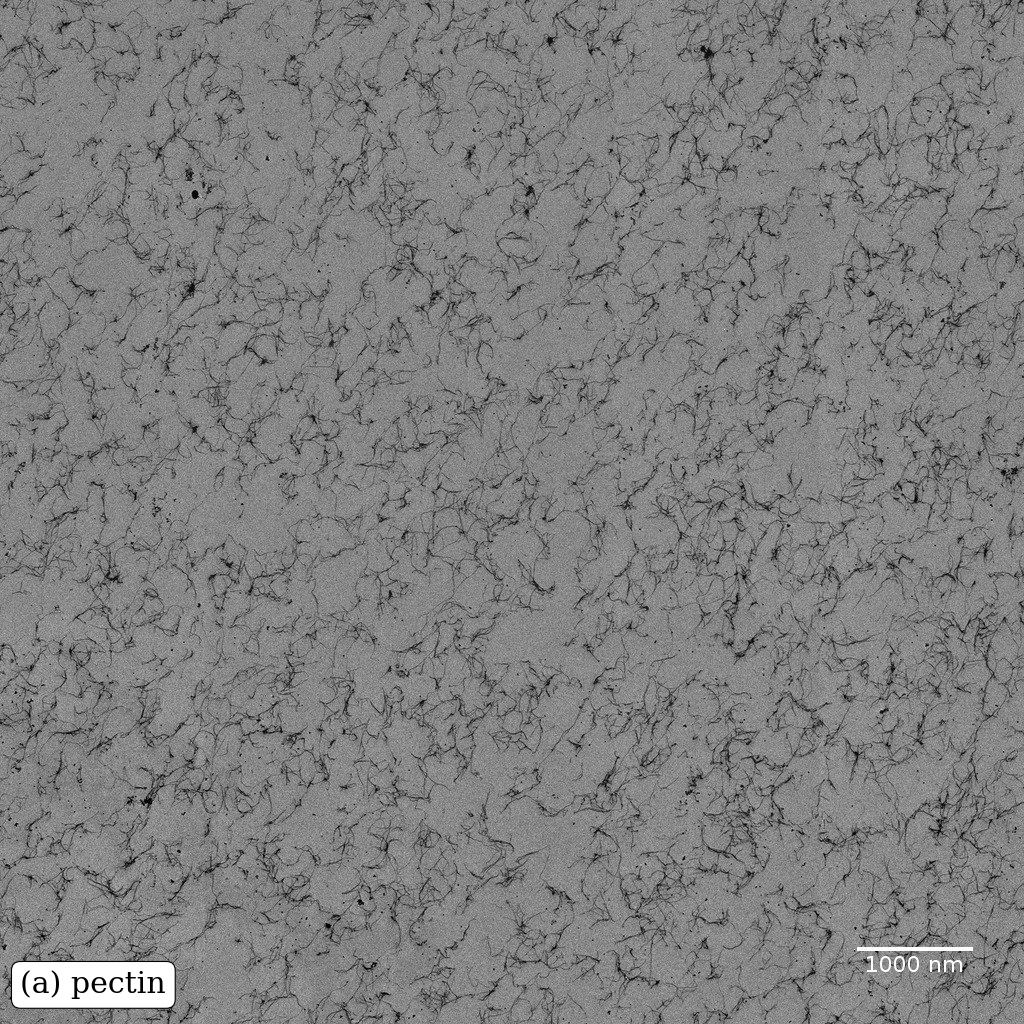
\includegraphics[width=0.32\textwidth]{Figures/chapter-temsaxs/pectin1_1045_homogeneous_scalebar_label.jpeg}
    \hspace{0.5pt}
    % \includegraphics[width=0.325\textwidth]{Figures/chapter-temsaxs/carrageenan_K_Montage_832_scalebarFixed_label.jpeg}
    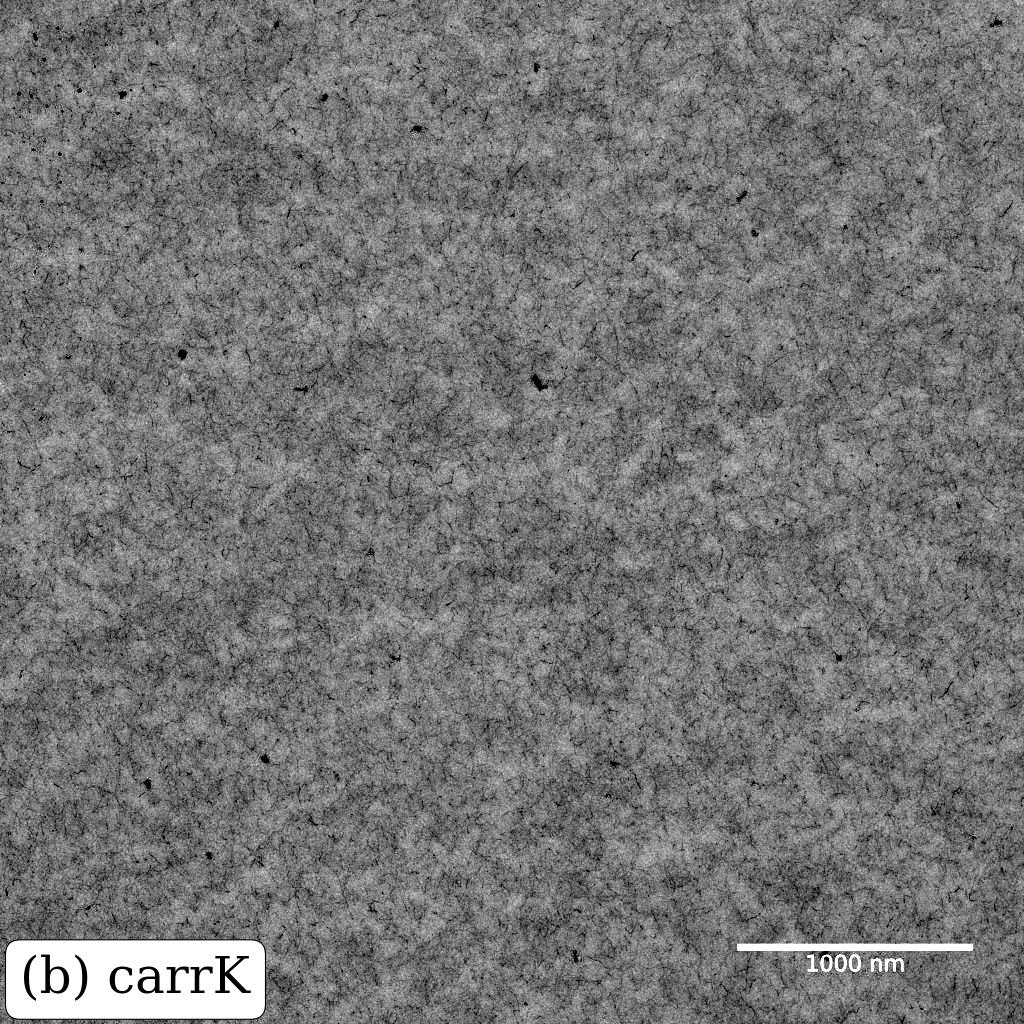
\includegraphics[width=0.32\linewidth]{Figures/chapter-temsaxs/carrageenan_K_Montage_833_scalebarFixed_normalized_label.jpeg}
    \hspace{0.5pt}
    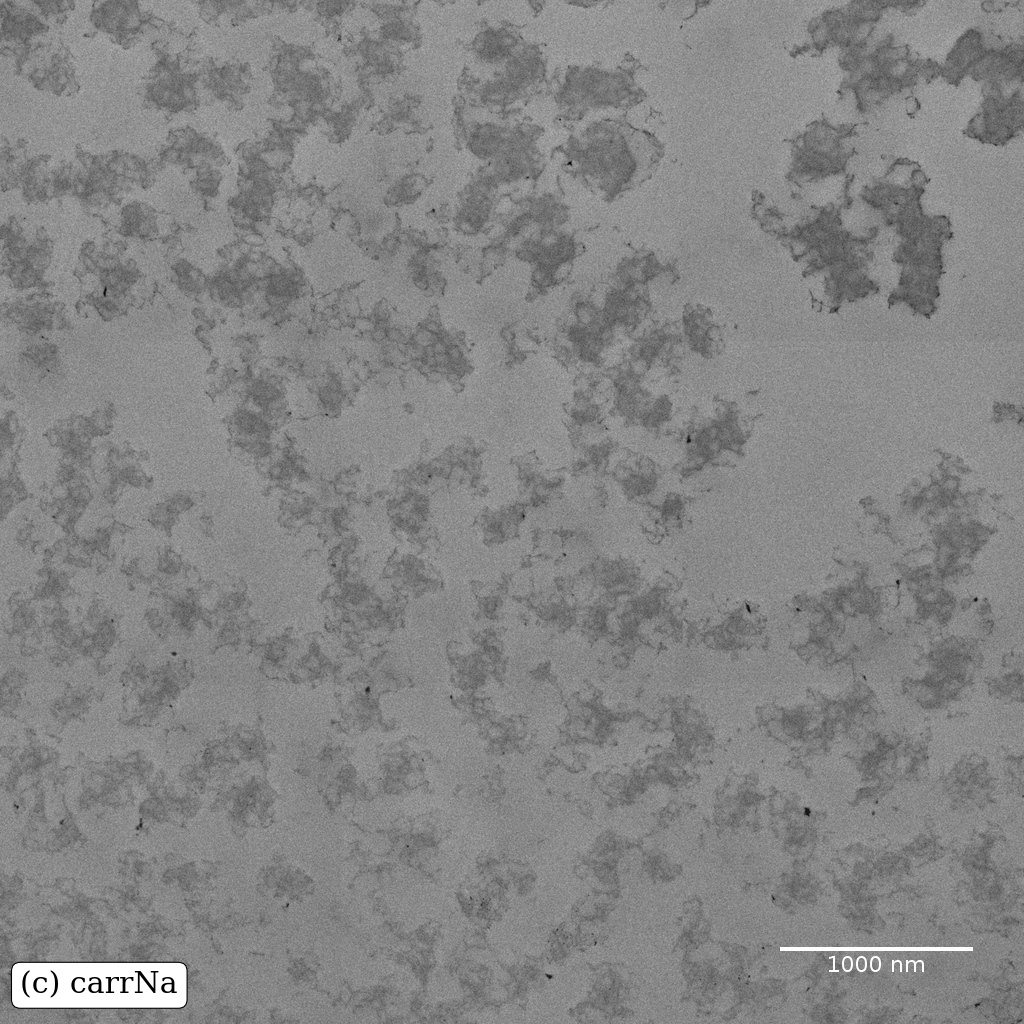
\includegraphics[width=0.32\textwidth]{Figures/chapter-temsaxs/carrageenan_Na_Montage_851_scalebar_label.jpeg}
    \caption{Montages of TEM images obtained from different polysaccharides, as described in the text.}\label{fig:fig1}
\end{figure*}


\subsection{Qualitative Structural Features}
The most striking difference between the three TEM images is the dense cluster-like associations seen in the sodium carrageenan gel, while the other networks show architectures built from more primitive rod-like structures. The self similarity of these cluster-like associations can be quantified by applying fractal analysis to the corresponding scattering data, whereupon the slope of a log-log plot of the scattered intensity versus q reveals the average fractal dimension of the scatterers in the sample. The SAXS data is shown in figure \ref{fig:SAXS} for the three samples together with a power-law fitting for the different regimes where self-similarity was observed. For the sodium carrageenan sample a low-q, a large length-scale, fractal dimension of ($1.93 \pm 0.02$), an intermediate-q fractal dimension of ($2.39 \pm 0.01$), and a high-q fractal dimension of ($2.11 \pm 0.02$) were measured. The similar fractal dimensions obtained across all measurable length scales testifies to the self similarity of this network over an extended distance range in good agreement with the microscopy. In contrast, the TEM images from the pectin and the potassium carrageenan networks both exhibit rod-like features in the micrographs. Correspondingly the SAXS data in the mid-q fractal regions do exhibit concomitant fractal dimensions of close 1, indicating the presence of rod-like features. Indeed, least-squares fitting reveals mid-q fractal dimensions of  ($1.27 \pm 0.01$) for pectin and ($1.12 \pm 0.01$) for carrageenan respectively, with the slight deviations from unity indicating some flexibility in the rod-like regions.    

\begin{figure}[H]
    \centering
    \noindent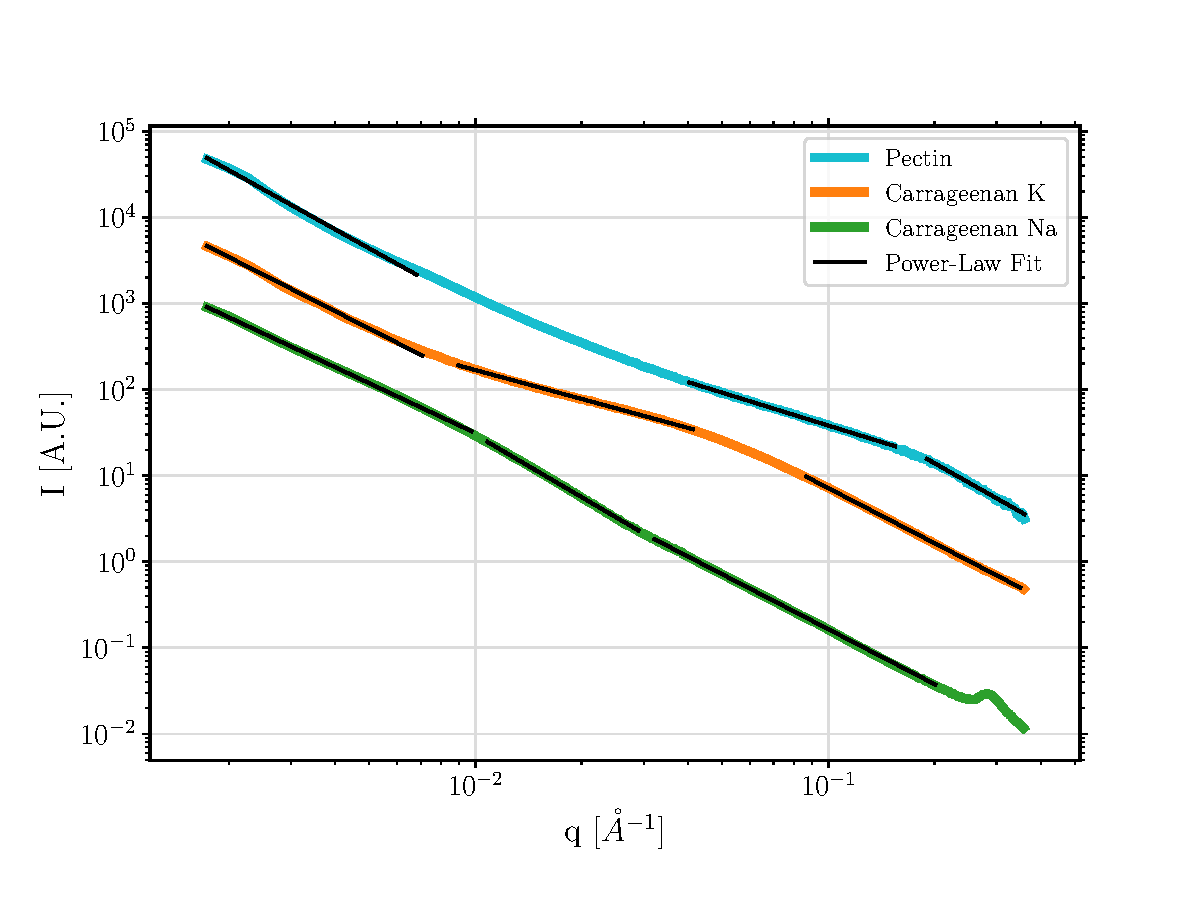
\includegraphics[width=0.75\linewidth]{Figures/chapter-temsaxs/saxs_fit.pdf}
    \caption{SAXS results for the three samples shown in the TEM micrographs of figure~\ref{fig:fig1}, in the absence of TEM sample preparation. Black lines signify power law fitting, as is described in section 3.1 of the text.}\label{fig:SAXS}
\end{figure}

\subsection{Consistency Between Techniques at Different Lengthscales}

Figure~\ref{fig:TEM_vs_SAXS} shows the reciprocal space data obtained by Fourier transformation of the montages presented in figure~\ref{fig:fig1}, for all three gelled systems, compared with the experimentally measured SAXS results. The absolute magnitude of the calculated data has been scaled in order to match as closely as possible that obtained from the experimental SAXS data. It should be noted that when performing the SAXS experiments, data is averaged over the scattering volume determined by the beam and cell geometry, roughly 0.2$\times$0.2$\times$1.5 \si{\mm^3}, and that by using combinations of camera lengths and beam-line energies, scattering vectors $q$ ranging between $[0.001, 1]$ \si{\nm^{-1}} (corresponding to approximately $[ 600, 0.6]$ \si{nm}) are routinely available at synchrotron facilities.


It can be seen that above $\sim$20 nm there is remarkably good agreement between the results obtained for all three samples, over the range of different polymers and network architectures (even when displayed on a logarithmic scale). This suggests that the electron microscopy sample preparation method as described herein is minimally perturbing to results in this size range and that TEM provides visual and SAXS-consistent information on the architecture of polysaccharide networks. The extraction of the statistical properties of such architectures forms part of our current work and will be reported elsewhere. Below 20 nm however it appears that there are substantial differences in the SAXS and TEM-derived reciprocal space representations, at least in two of the gels. Given that the SAXS data represent the unperturbed gels, this suggests that analysis by classical transmission electron microscopy is not suitable for structural studies of polysaccharide gels at the level of filaments and their supramolecular arrangements. It can be hypothesized that such deviations are brought about by some combination of fixing, contrasting and plastic embedding of the networks, and/or changes to the resin that occur during exposure to the electron beam. The dehydration step during which the gel is exposed to increasing concentrations of ethanol leads to a deswelling of the network which, given the miscibility of ethanol and water, is believed to be isotropic in nature. It is worth pointing out that the structural distortions to the network due to beam exposure seem to be relatively small in comparison to the structural changes during dehydration. 

Exposure of the epoxy-embedded section to the electron beam is known to cause anisotropic shrinkage in the x-y plane of the resin-embedded specimen section \cite{luther_sample_2007}, while mass loss due to outgassing of the polymer resin in vacuum causes collapse of the volume orthogonal to the beam. Together, these beam-induced distortions are known to be complex, and they cannot be corrected by simple stretching factors that address only isotropic distortions. According to our measurements, the distortions observed at length scales > 20 nm appear to be remarkably isotropic, indicating that the end result of the sample preparation steps prior to imaging (dehydration, embedding, beam-induced changes) either cause negligible change to the gel structure or more probably, a change of some magnitude that is directly proportional to the native structure as shown by SAXS. This means that any quantification of the accumulated changes that occur during EM sample preparation and analysis can be applied to the final micrographs with confidence. Importantly, the same does not apply to length scales < 20nm, where the electron-dense reagents used to provide amplitude contrast are unlikely to be a perfect approximation of the fibre structure. Indeed the specificity of Ruthenium Red is not clear and even a single hexavalent cation has a diameter of approximately 1.13 nm \cite{chaffey_principles_2001}. Furthermore, post-staining with uranyl acetate was found to be necessary to facilitate image analysis. These observations suggest that the contrast agents are a primary source of discrepancies between TEM and SAXS at the level of the network strands.

Cryo- electron microscopy of vitrified gels would conceivably solve some of these sample preparation and imaging issues, and may yet prove useful in investigating the fine structure of polysaccharide networks; however, cryo sample preparation (which circumvents the need for chemical fixatives, dehydration and staining) must as a minimum contend with the naturally high water content of the gels, which makes vitrification challenging. Furthermore, polysaccharides are poor phase objects compared to e.g. proteins, making it difficult to generate the image signal-to-noise characteristics required for computational analysis of network fine structure. If vitrification of the gel was physically possible, cryo- negative staining would avoid all of the problems mentioned except for non-natural contrast. As reported in this study, the (predominantly amplitude) contrast generated by classical TEM is due to the stain rather than the fibers, and the validity of this technique at high resolution depends increasingly on the stain representing a faithful approximation of the fiber structure. Given the fact that vitrification of these gels is likely to be very difficult to achieve, we suggest that computational methods based on unwarping of the distorted structure (based on the movements of fiducial markers, for example), will be more useful in interrogating the fine structure with the required level of accuracy. If, however, staining artifacts contribute significantly to the inaccuracies, consideration must be given to imaging the natural phase contrast of unstained fibers.

\begin{figure}[!ht]
    \centering
    \noindent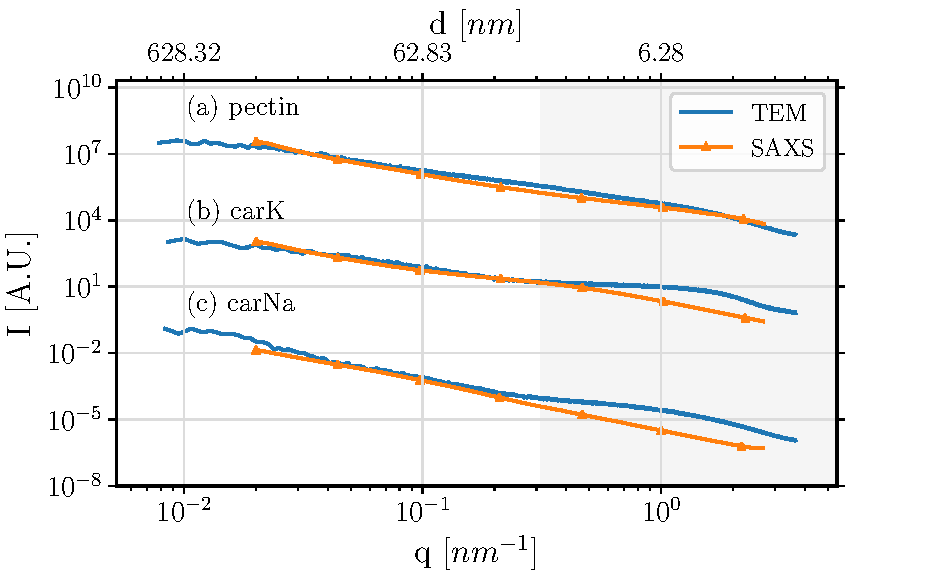
\includegraphics[width=0.95\linewidth]{Figures/chapter-temsaxs/saxs-tem-merged.pdf}
    \caption{Comparison of data obtained from TEM best practice and SAXS. Good agreement can be seen in the large network scale (at low $q$s). The shaded area shows the upper $q$ range (smaller than 20 \si{\nm} or equivalently 25 pixels). The top x-axis shows the corresponding real-space length scale, where $d = 2\pi/q$.} \label{fig:TEM_vs_SAXS}
\end{figure}

\subsection{Image Processing}
The effect of de-noising algorithms commonly used to aid in the extraction and segmentation of network architectures, and in a range of broader image processing applications has also been investigated. In particular, the use of a total variation (TV) regularization \cite{barbero_fast_2011, barbero_modular_2014} and a wavelet based BLS-GSM algorithm \cite{portilla_image_2003, rajaei_analysis_2014, hernandez-cerdan_isotropic_2017} have been investigated. These filters are anisotropic and attempt to reduce noise present in the high frequency domain, while conserving edges of the regions of interest. The adjustable parameters that are manipulated in these algorithms, routinely referred to as lambda in TV, and sigma in BLS-GSM, were chosen in order to achieve the most significant reduction of high frequency speckles, while avoiding blurring or modification of the high intensity structures.
Figure~\ref{fig:fig3} shows the analysis in the reciprocal space of the de-noised images, and reveals that while the application of the TV algorithm in particular appears to improve the consistency of the TEM and SAXS data towards lower length-scales still, especially for the carrageenan networks, significant modification of the small-length data ($<$20\si{\nm}) is produced through image processing, indicating that the information obtainable from TEM below this length-scale is not so robust and should indeed be treated with caution. On a positive note, the data in the large-length (low-frequency range) is largely unaffected by the application of these algorithms and still agrees with that recorded using SAXS. An example of the effects of de-noising in real-space is shown in Figure~\ref{fig:denoised_images}.

\begin{figure*}[!ht]
  \begin{minipage}{0.32\textwidth}
    % \noindent\includegraphics[width=\linewidth]{./figs-tikz/saxs-tem-TV-pectin.svg}\label{fig:denoise_pectin_image}

    \noindent\includegraphics[width=\linewidth]{Figures/chapter-temsaxs/saxs-tem-TV-pectin.pdf}\label{fig:denoise_pectin}
  \end{minipage}
  \begin{minipage}{0.32\textwidth}
    % \includegraphics[width=\linewidth]{./figs-tikz/saxs-tem-TV-carK.svg}\label{fig:denoise_carrK_image}

    \includegraphics[width=\linewidth]{Figures/chapter-temsaxs/saxs-tem-TV-carK.pdf}\label{fig:denoise_carrK}
  \end{minipage}
  \begin{minipage}{0.32\textwidth}
    % \includegraphics[width=\linewidth]{./figs-tikz/saxs-tem-TV-carNa.svg}\label{fig:denoise_carrNa_image}

    \includegraphics[width=\linewidth]{Figures/chapter-temsaxs/saxs-tem-TV-carNa.pdf}\label{fig:denoise_carrNa}
  \end{minipage}
  \caption{
    Results obtained when applying two widely-used de-noising techniques: total variation regularization (TV) and multi-scale wavelet denoising using a BLS-GSM algorithm.}
\label{fig:fig3}
\end{figure*}

\begin{figure*}[!ht]
  \begin{minipage}{0.32\textwidth}
    \noindent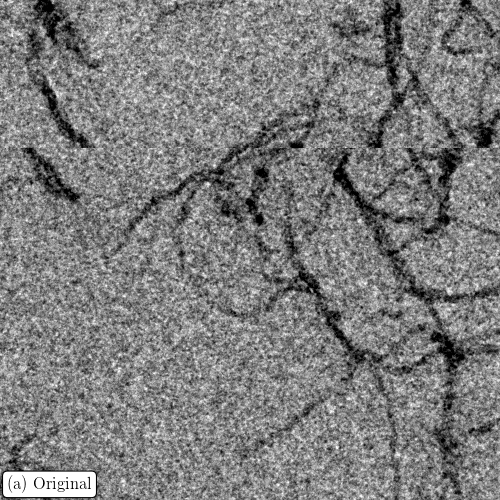
\includegraphics[width=\linewidth]{Figures/chapter-temsaxs/pectin_crop_tile01_500x500_900_1900_label.png}\label{fig:denoise_comparison_pectin_original}
  \end{minipage}
  \begin{minipage}{0.32\textwidth}
    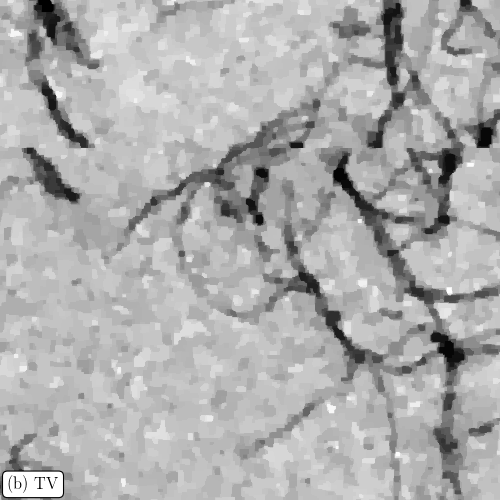
\includegraphics[width=\linewidth]{Figures/chapter-temsaxs/pectin_TV_lam015_crop_tile01_500x500_900_1900_label.png}\label{fig:denoise_comparison_pectin_TV}
  \end{minipage}
  \begin{minipage}{0.32\textwidth}
    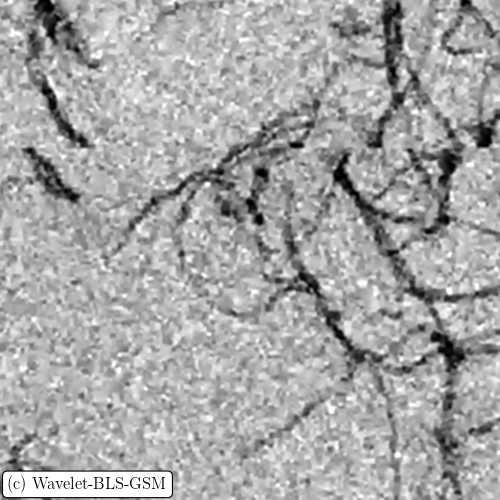
\includegraphics[width=\linewidth]{Figures/chapter-temsaxs/pectinPortillaSigma28_crop_tile01_500x500_900_1900_label.png}\label{fig:denoise_comparison_pectin_wavelet}
  \end{minipage}
  \caption{Visual comparison of the de-noised pectin TEM images (Fig~\ref{fig:fig1}a). (a) shows a region from the unmodified original image, (b): de-noised image using a total variation method \cite{barbero_modular_2014} with $\lambda = 0.15$, (c) shows the same region after applying a multi-scale wavelet approach using the BLS-GSM algorithm \cite{portilla_image_2003} with $\sigma = 28.4$. Only high-frequency regions are affected by de-noising algorithms, as reflected in the generated I-q plots shown in Fig~\ref{fig:fig3}a.
}\label{fig:denoised_images}
\end{figure*}


\subsection{Extracting Persistence Lengths}
In order to investigate the possible quantitative extraction of persistence lengths from the TEM images acquired (Fig~\ref{fig:fig1}) they were analyzed directly using FiberApp \cite{usov2015}. This open-source software, available for tracking and analyzing polymers, filaments, biomacromolecules and fibrous objects, was used to estimate the persistence lengths of the network filaments. Figure~\ref{fig:fig5} shows the application of FiberApp to one of the acquired TEM images and the extraction of a persistence length for the polymer chains between junction zones. While the algorithm itself works well, as demonstrated by the quality of the fit of the data to the worm-like chain model (Figure~\ref{fig:fig5} (Insert)) a persistence length of some 140 nm is recovered. In contrast, fitting the corresponding scattering data acquired by SAXS experiments recovers a value of almost an order of magnitude less then this. (Specifically, SAXS results from such pectin acid gels have been fitted previously to a model of flexible cylinders arranged according to a fractal structure factor \cite{mansel_zooming_2015} and Kuhn lengths of around 9.75 nm were obtained.) Considering that the scattering-determined value of the persistence length of the chains in this polysaccharide network is less than $\sim$20 nm, the fact that the value found in the samples prepared for TEM is different is consistent with out contention that while features of the unadulterated networks above $\sim$20 nm are largely unaffected by the significant preparation procedure, smaller features can be significantly perturbed.


It can be hypothesized that such changes in the measured stiffness of the filaments are brought about by fixing, labeling and finally plastic embedding of the networks. It hardly seems surprising that in a situation where the dielectric constant of both the alcohols used for exchange and the final embedding resin are significantly less than water, and indeed where the mechanical properties of the embedding resin when cured are significant that the original thermal fluctuations of the network fibers are now significantly hindered. 

\begin{figure}[!ht]
    \centering
    \noindent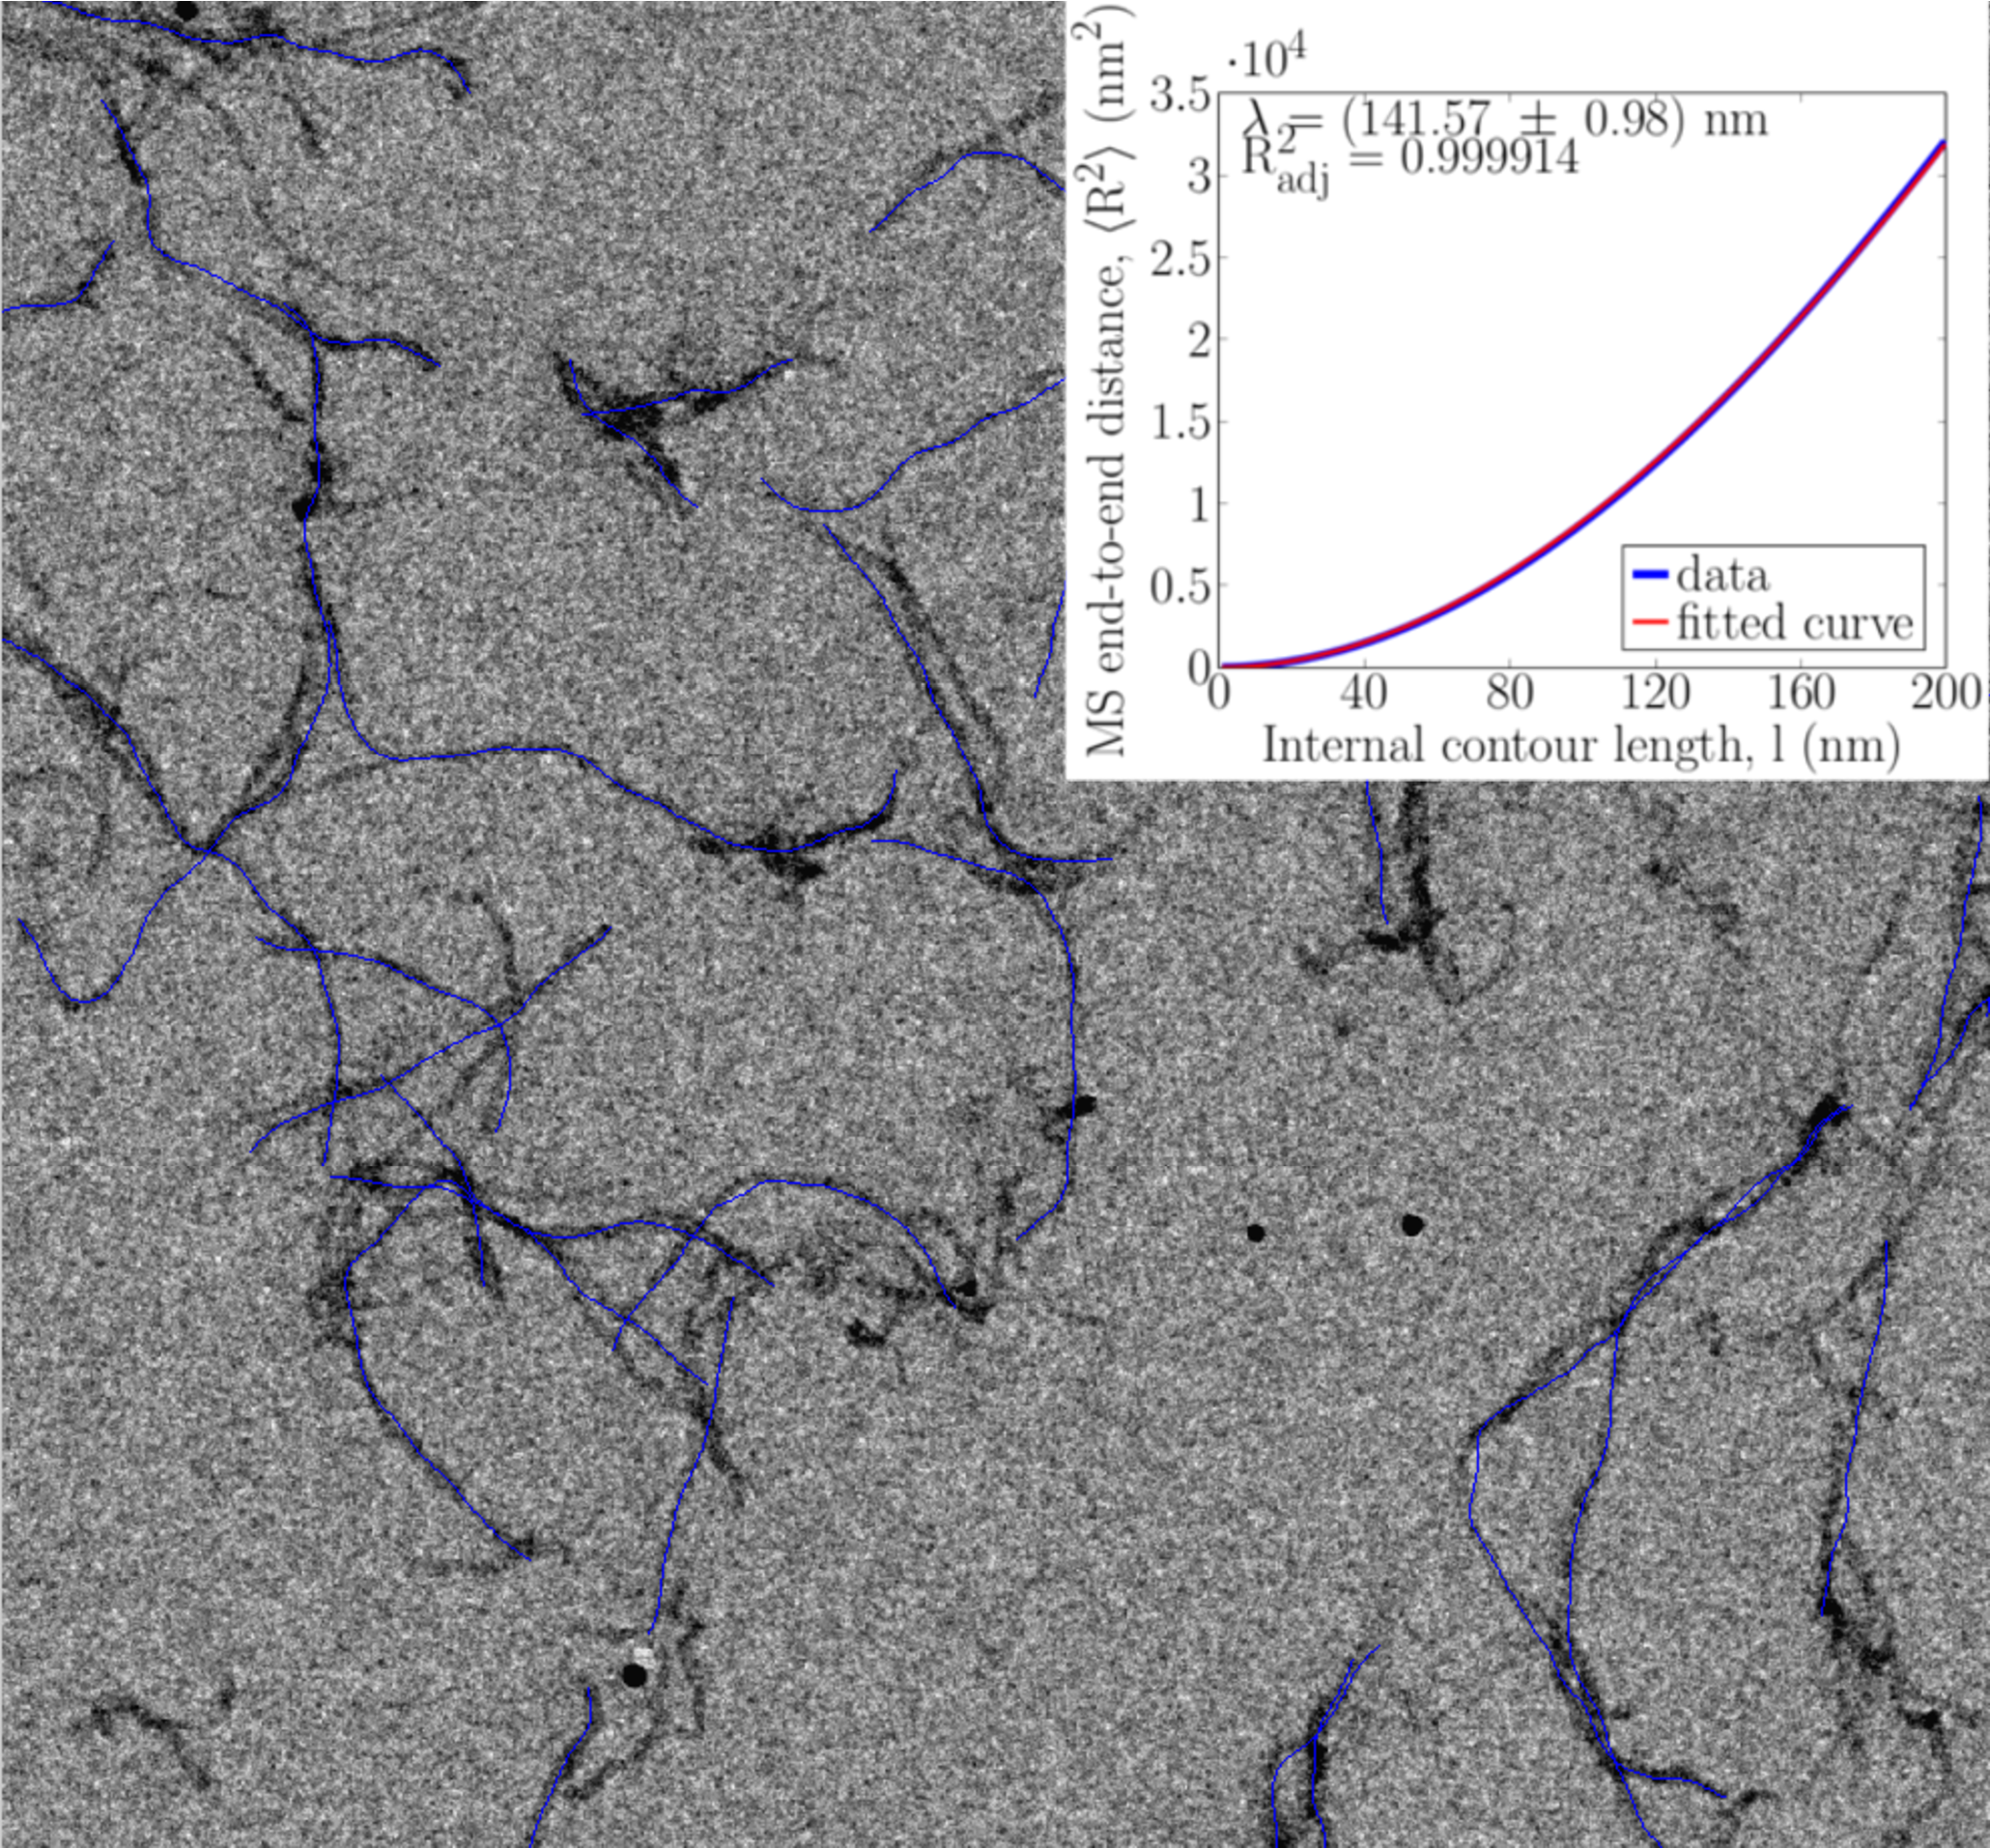
\includegraphics[width=0.7\linewidth]{Figures/chapter-temsaxs/fibreAppTrackingImage_subplot.pdf}
    \caption{A TEM micrograph with FibreApp tracking output shown in blue. The insert shows the internal contour length vs mean-square end-to-end distance calculated from the corresponding tracking parameters.}\label{fig:fig5}
\end{figure}


\section{Conclusions}
The structures of three different polysaccharide networks have been studied over length scales from 1 nm to many microns, using SAXS and TEM imaging, revealing marked differences between gels and consistency between techniques at a resolution > 20nm. The networks exhibit different exemplary architectures: the sodium carrageenan gel is fractal in nature (consistent with polyelectrolytic condensation) while in contrast the potassium carrageenan and pectin samples were comprised of more homogeneous rod-like elements (consistent with the more specific interactions). The studies carried out here show that despite the fact that extensive sample preparation is needed to plastic-embed samples for TEM, careful protocols can produce datasets where information acquired above around 20 nm is consistent with that obtained by SAXS studies carried out on unadulterated samples. Information regarding chain thicknesses and flexibilities are clearly modified by labeling and by changes in the dielectric constant and mechanical properties of the surroundings, manifesting discrepancies between the results of the techniques. Further work is planned to characterise the network structure using SAXS during the sequence of TEM preparation steps, i.e. fixation and dehydration. These experiments will elucidate the structural changes induced by the TEM sample preparation and the results will guide new strategies for sample preparations with the aim to reduce the induced structural changes and enhance the image quality, leading to reduced requirements for image processing. However, the fact that at larger length scale the structure of the pre-prepared water-rich networks seem largely preserved in the TEM samples suggests that 3D TEM tomography experiments carried out with careful sample preparation will be valuable tools for measuring network architecture and connectivity; information that is lost in SAXS owing to the intrinsic averaging nature of the technique. 
 

The authors acknowledge the New Zealand Synchrotron group for funding for the SAXS experiments, and the MacDiarmid institute for PhD studentships (PHC, BWM), and 
Raffaele Mezzenga, Niklas Lor{\'e}n and Annika Altsk{\"a}r for interesting discussions.
